\chapter{Implementation and User Interface}
		
		\section{Used technologies and tools}
		
		We have developed a mobile application for the Android operating system. The IDE of choice was Android Studio\footnote{\url{https://developer.android.com/}}. We have chosen it because it was developed by Google who are considered to be a sort of authority on Android. On the back-end we used Python\footnote{\url{https://www.python.org/}} hosted on the cloud at the site Pythonanywhere\footnote{\url{https://www.pythonanywhere.com/user/kaogrupa/}}.
		
		The database was also hosted on the aforementioned cloud. The database of choice was SQLite3\footnote{\url{https://www.sqlite.org/index.html}}. The pythonanywhere cloud offered the ability to start shell consoles and from there manage the database, as well as edit the Python back-end files. The back-end was made in Python Flask\footnote{\url{https://palletsprojects.com/p/flask/}} - a micro web framework. The cloud made the deployment and integration seamless and easy.
		
		Flask cooperates with further sub-components(as visible in the component diagram) - SQLAlchemy\footnote{\url{https://www.sqlalchemy.org/}}, Flask-JWT\footnote{\url{https://pythonhosted.org/Flask-JWT/}}, and Marshmallow\footnote{\url{https://marshmallow.readthedocs.io/en/stable/}}. SqlAlchemy is the component used for communicating with the database, JWT is used for the OAuth 2.0 implementation\footnote{\url{https://oauth.net/2/}}, and Marshmallow is used for JSON serialisation and de-serialisation. JWT = JSON Web Token.
		
		Front-end design and logic were all developed in Android Studio which provided a very convenient IDE --> code-generation and assistance was of great help, as well as the ability to edit XML files through a GUI instead of only the classical text editing. The application can be deployed and/or debugged on the mobile device by connecting it to the PC/Mac that has Android Studio running with the application code loaded into it. This has provided the basis for smooth application development and testing.
		
		Team communication was at first achieved using the Whatsapp application.\footnote{\url{https://www.whatsapp.com//}}. This worked at first, but has since proven itself to not provide satisfactory level of organisation and communication features. Therefore it was replaced with Slack\footnote{\url{https://slack.com/}} - where multiple threads and channels have made organisation and project overview much easier. What's more, a Slack bot and tasks have further increased the productivity and organisation.
		
		The version control system used was Git\footnote{\url{https://git-scm.com/}}. The most important branches were: master, dev, and devdoc. The application code was put on the dev branch, while the documentation resided on the devdoc branch. Before turning the application in, branched would be merged to the main branch --> the master branch. 
		
		The software used for documentation were: LaTeX\footnote{\url{https://www.latex-project.org/}} and Astah UML\footnote{\url{http://astah.net/}}. For LaTeX, we were provided with a template which greatly helped with LaTeX understanding and documentation writing. Astah UML was used for drawing diagrams and ha proven to be very accessible, intuitive, and satisfying to use.
		
		\eject 
	
		\section{Ispitivanje programskog rješenja}
			
			\textbf{\textit{dio 2. revizije}}\\
			
			 \textit{U ovom poglavlju je potrebno opisati provedbu ispitivanja implementiranih funkcionalnosti na razini komponenti i na razini cijelog sustava s prikazom odabranih ispitnih slučajeva. Studenti trebaju ispitati temeljnu funkcionalnost i rubne uvjete.}
	
			
			\subsection{Ispitivanje komponenti}
			\textit{Potrebno je provesti ispitivanje jedinica (engl. unit testing) nad razredima koji implementiraju temeljne funkcionalnosti. Razraditi \textbf{minimalno 6 ispitnih slučajeva} u kojima će se ispitati redovni slučajevi, rubni uvjeti te izazivanje pogreške (engl. exception throwing). Poželjno je stvoriti i ispitni slučaj koji koristi funkcionalnosti koje nisu implementirane. Potrebno je priložiti izvorni kôd svih ispitnih slučajeva te prikaz rezultata izvođenja ispita u razvojnom okruženju (prolaz/pad ispita). }
			
			
			
			\subsection{Ispitivanje sustava}
			
			 \textit{Potrebno je provesti i opisati ispitivanje sustava koristeći radni okvir Selenium\footnote{\url{https://www.seleniumhq.org/}}. Razraditi \textbf{minimalno 4 ispitna slučaja} u kojima će se ispitati redovni slučajevi, rubni uvjeti te poziv funkcionalnosti koja nije implementirana/izaziva pogrešku kako bi se vidjelo na koji način sustav reagira kada nešto nije u potpunosti ostvareno. Ispitni slučaj se treba sastojati od ulaza (npr. korisničko ime i lozinka), očekivanog izlaza ili rezultata, koraka ispitivanja i dobivenog izlaza ili rezultata.\\ }
			 
			 \textit{Izradu ispitnih slučajeva pomoću radnog okvira Selenium moguće je provesti pomoću jednog od sljedeća dva alata:}
			 \begin{itemize}
			 	\item \textit{dodatak za preglednik \textbf{Selenium IDE} - snimanje korisnikovih akcija radi automatskog ponavljanja ispita	}
			 	\item \textit{\textbf{Selenium WebDriver} - podrška za pisanje ispita u jezicima Java, C\#, PHP koristeći posebno programsko sučelje.}
			 \end{itemize}
		 	\textit{Detalji o korištenju alata Selenium bit će prikazani na posebnom predavanju tijekom semestra.}
			
			\eject 
			
		\section{UML Deployment Diagram}
		
			Due to the application including a lot of users, we have opted for the specification deployment diagram.
			The application consists of two parts: the mobile application(kind of a front-end) and the back-end hosted on the Pythonanywhere cloud. The application uses protocols GET(for information retrieval from the server), and POST in order to send/communicate information to the server. Furthermore, the server consists of 4 parts:
			\begin{itemize}
				\item App.db - definition of the database for SQLite 3
				\item Models.py - database tables modelled as Python classes
				\item Run.py - endpoint initialisation and control
				\item Resource.py - Used for handling server requests and responses
			\end{itemize}
			
			As far as hardware goes - basically 2 devices are required - the mobile phone and the cloud hosting computer. Network is also required as it is used to convey
			information between these 2 endpoints. While there is only one server instance, it is expected that multiple concurrent mobile phones will be using the application. Therefore, in the instance deployment diagram more than one mobile phone could be present.
		
			\begin{figure}[H]
				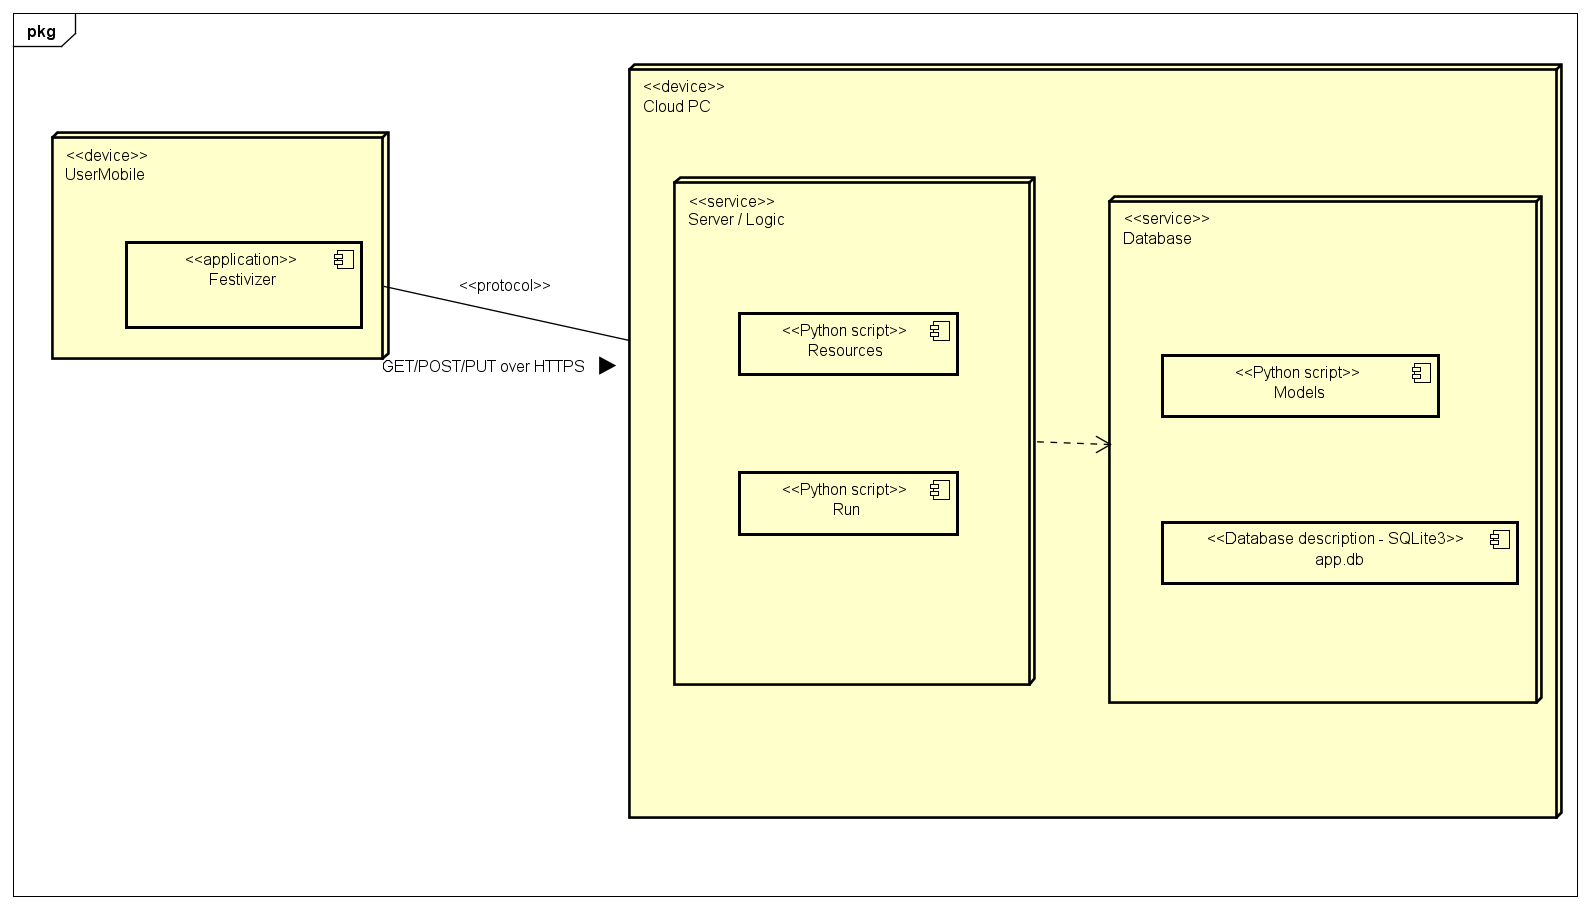
\includegraphics[width=\linewidth]{diagrams/Deployment Diagram0.png}
				\caption{Deployment Diagram}
				\label{fig:deployment_diag}
			\end{figure}
		
			\eject			
		\section{Deployment instructions}
			
			\subsection{Building the APK}
			
			The APK can be built in the following way:
			First, you need to git clone the application's repository: https://gitlab.com/barbil/organization_of_the_festival
			
			\begin{figure}[H]
				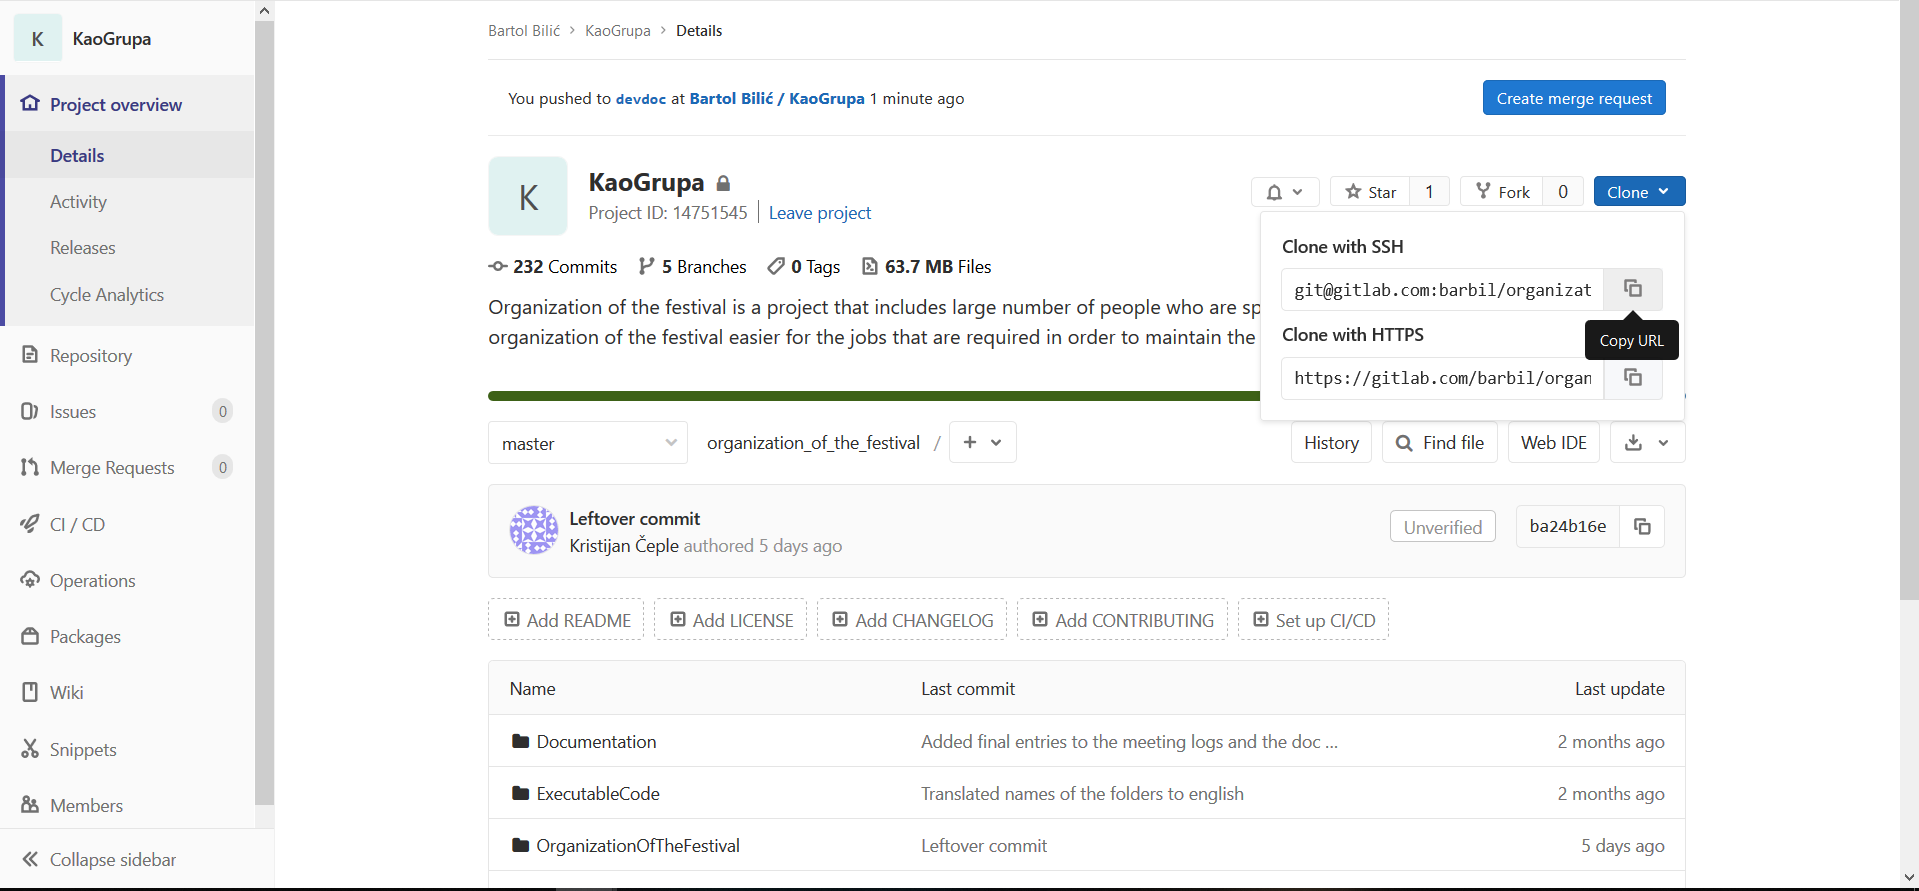
\includegraphics[width=\linewidth]{images/Deploy_M_1.png}
				\caption{Cloning from git}
				\label{fig:install_1}
			\end{figure}
			
			After pulling, the project needs to be opened in Android Studio. Merely go \textbf{File -> Open}, and then navigate to the cloned git repository. There you will find the project file that can be opened. Now, you would want to build an APK to run it on your device.
			
			\begin{figure}[H]
				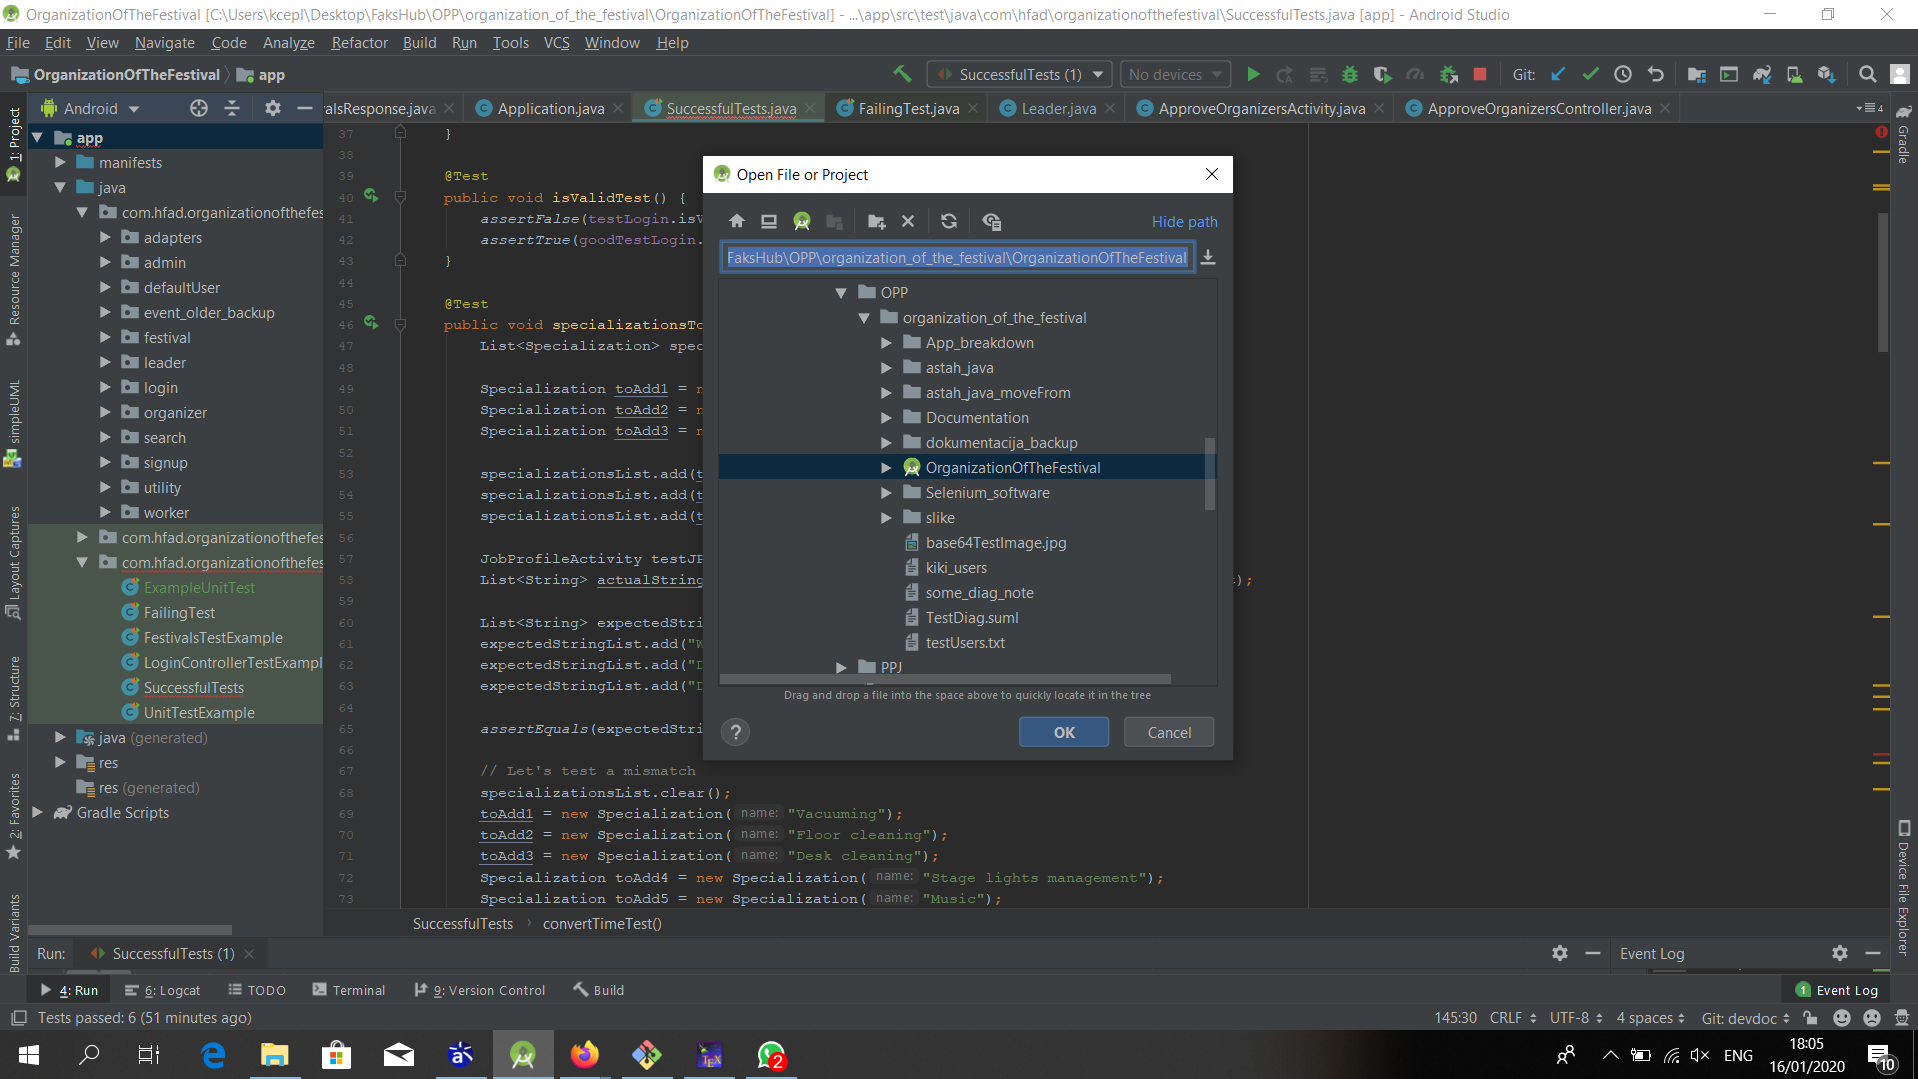
\includegraphics[width=\linewidth]{images/Deploy_M_2.png}
				\caption{Opening the Project}
				\label{fig:install_2}
			\end{figure}
			
			There is also an alternative. It is to go to our store, and install the app from there. Also, it is possible to build a signed build in Android Studio that is ready for deployment on any App store.
			
			Here, we will go into the process of generating your APK. Go to \textbf{Build -> Build Bundle(s)/APK(s)} or \textbf{Build -> Build Signed Bundle/APK}. If opting for signed bundles and APKs, you will need to generate a secure key that will be used for the signing process.
			
			\begin{figure}[H]
				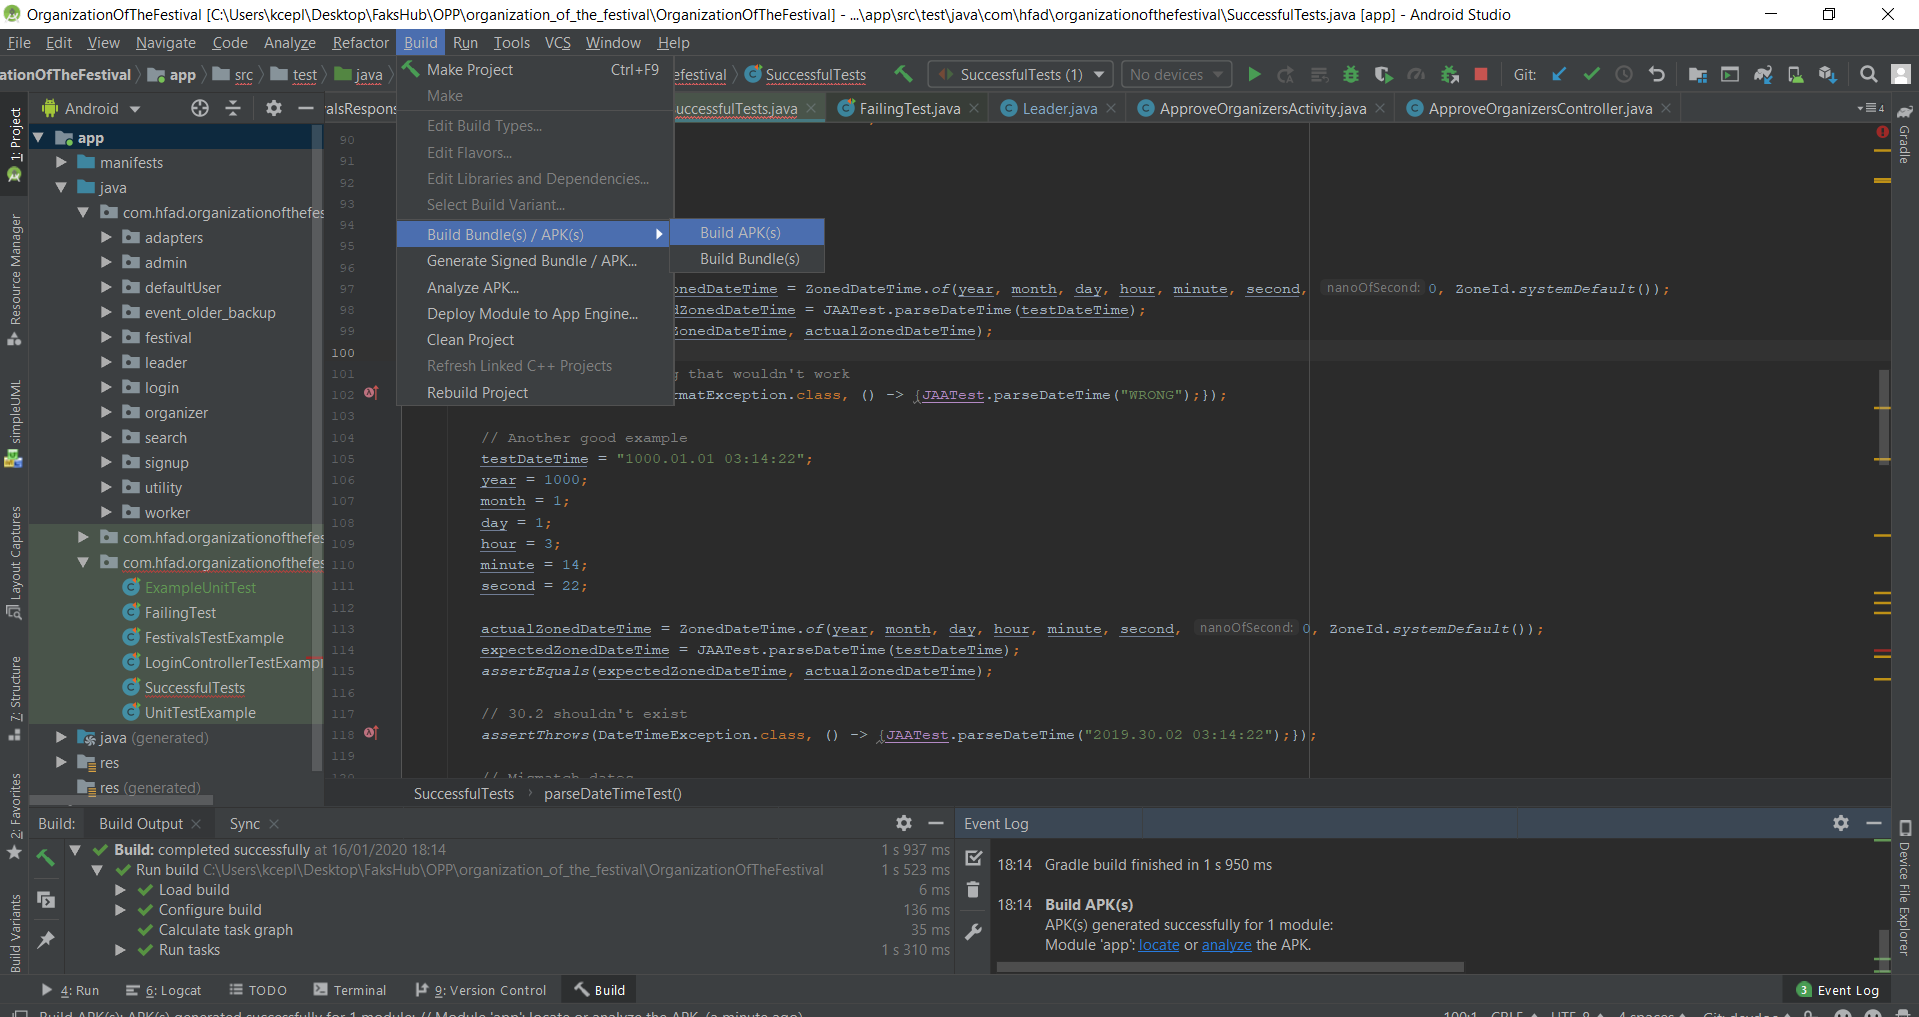
\includegraphics[width=\linewidth]{images/Deploy_M_3.png}
				\caption{Building process}
				\label{fig:install_3}
			\end{figure}
			
			\begin{figure}[H]
				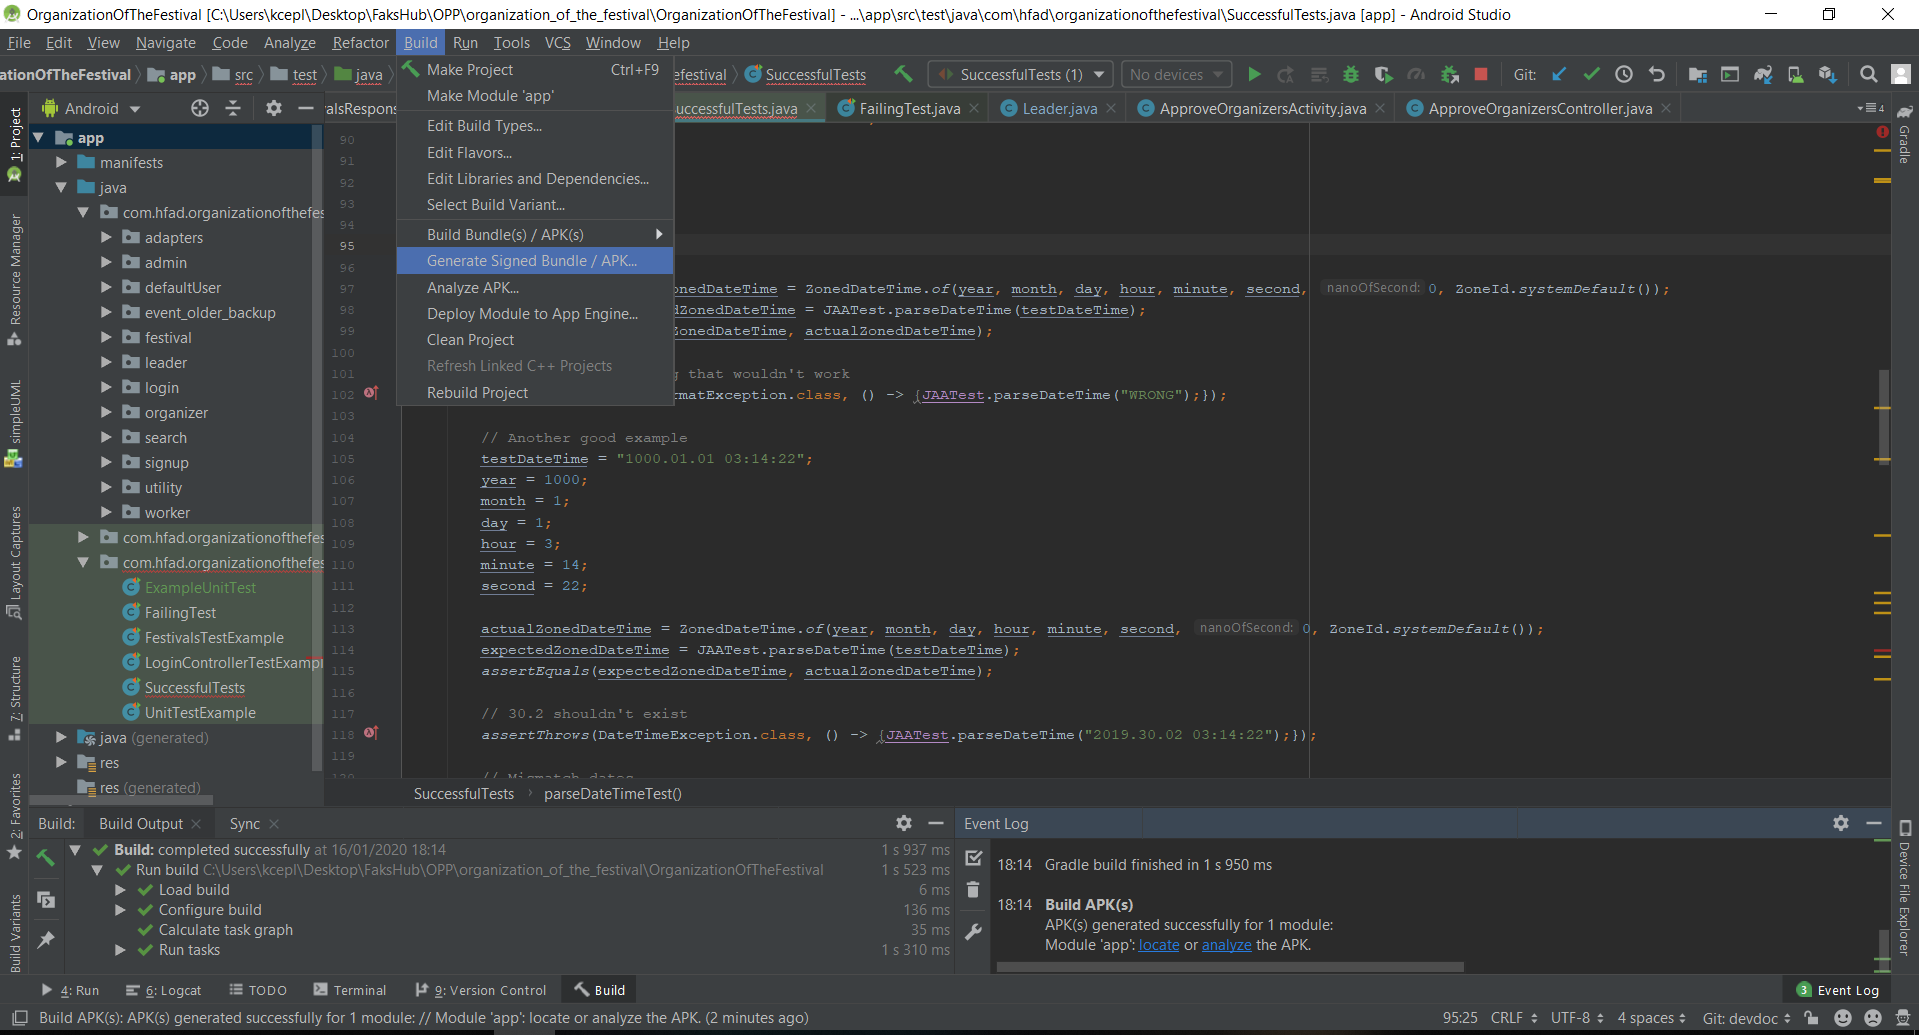
\includegraphics[width=\linewidth]{images/Deploy_M_4.png}
				\caption{Building process}
				\label{fig:install_4}
			\end{figure}
			
			\begin{figure}[H]
				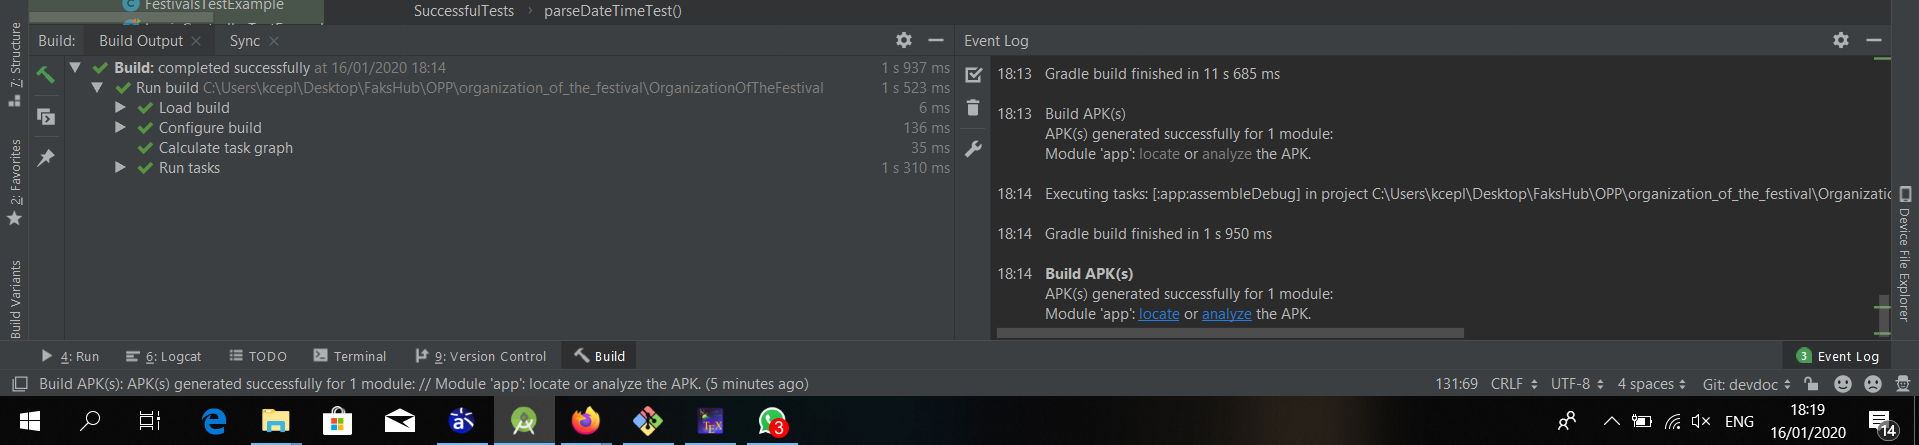
\includegraphics[width=\linewidth]{images/Deploy_M_5.png}
				\caption{Building process}
				\label{fig:install_5}
			\end{figure}
			
			Once you have the APK, it can be uploaded to any app store. \textbf{The APKs that will be uploaded to the app store SHOULD be signed.} It is also possible to put this .apk on the mobile device, and install it it there.
			
			Upon running the application, it will automatically connect to the kaogrupa pythonanywhere site, and communicate with the server. You are now ready to use the application. 2
			
			\subsection{Setting up the server side}
				
				The files are already present on the git URI, branch python_backend: https://gitlab.com/barbil/organization_of_the_festival/tree/python_backend. First of all this git should be cloned down somewhere. The files inside will be put onto the server. For deployment we used pythonanywhere as a cloud site, since it allows easy and seamless deployment of Flask applications.
				
				Second of all, you should either register or log in into pythonanywhere site.
				\begin{figure}[H]
					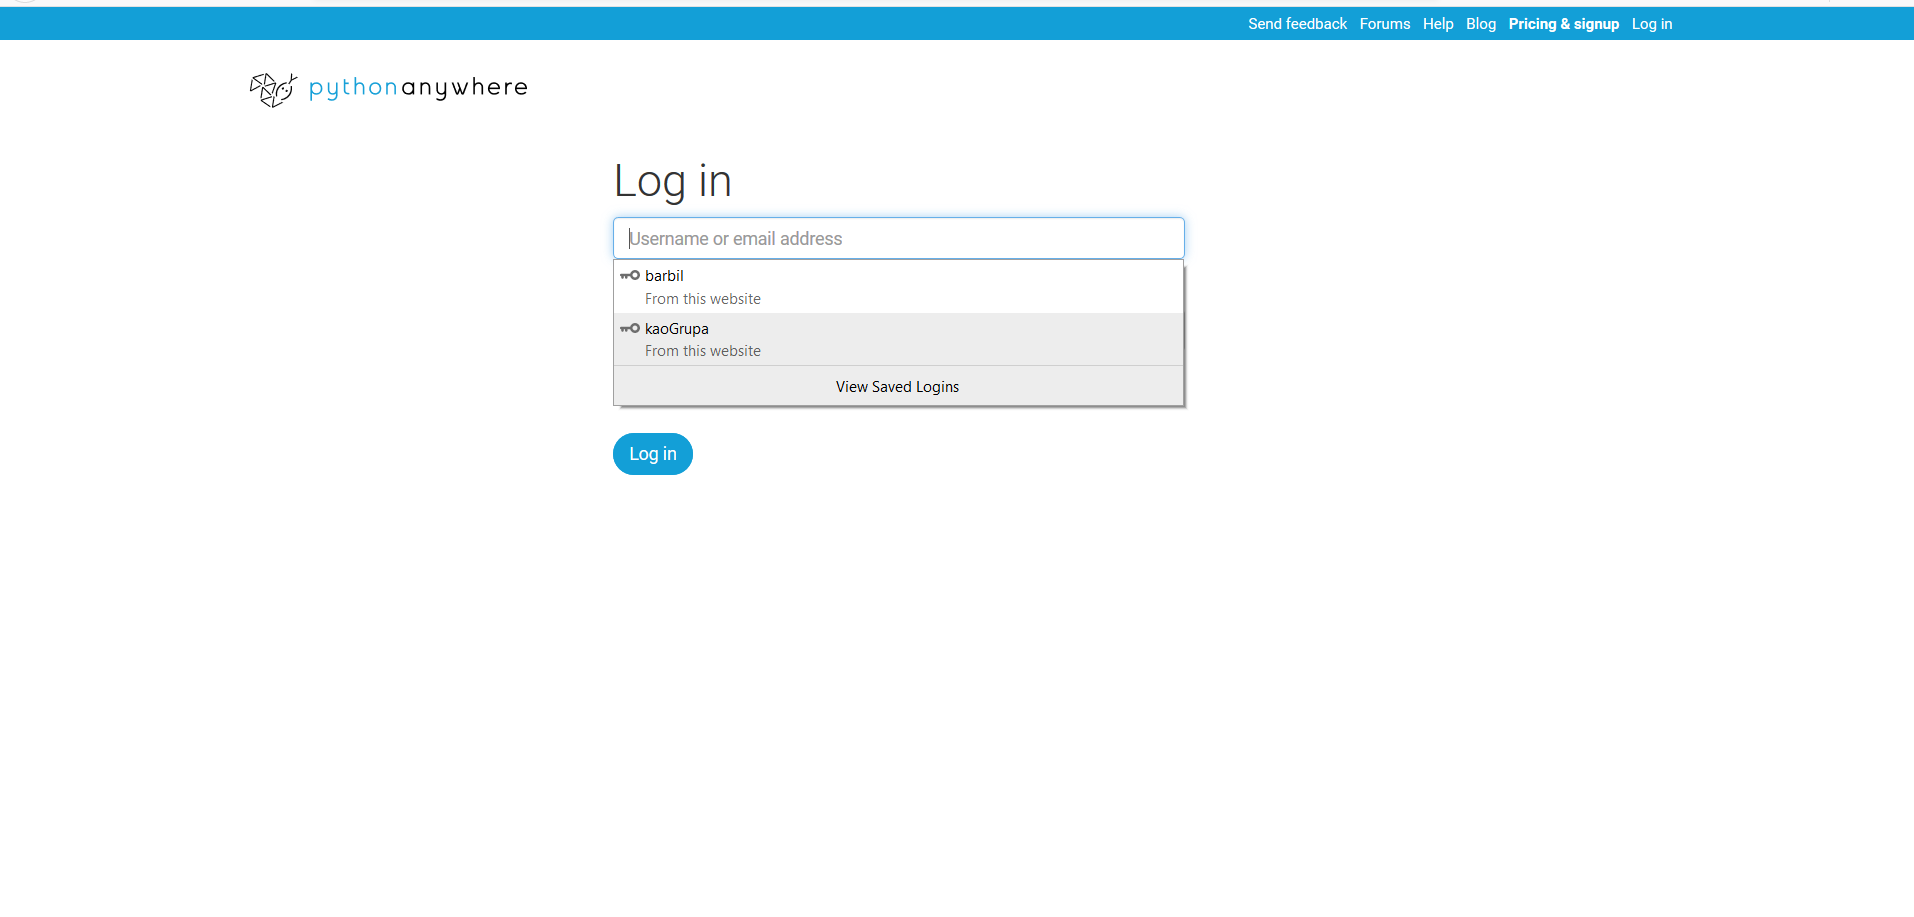
\includegraphics[width=\linewidth]{images/Deploy_1.png}
					\caption{Logging-In}
					\label{fig:deployment_1}
				\end{figure}
			
				Afterwards you should be taken to the dashboard screen. It should look something like this:
				\begin{figure}[H]
					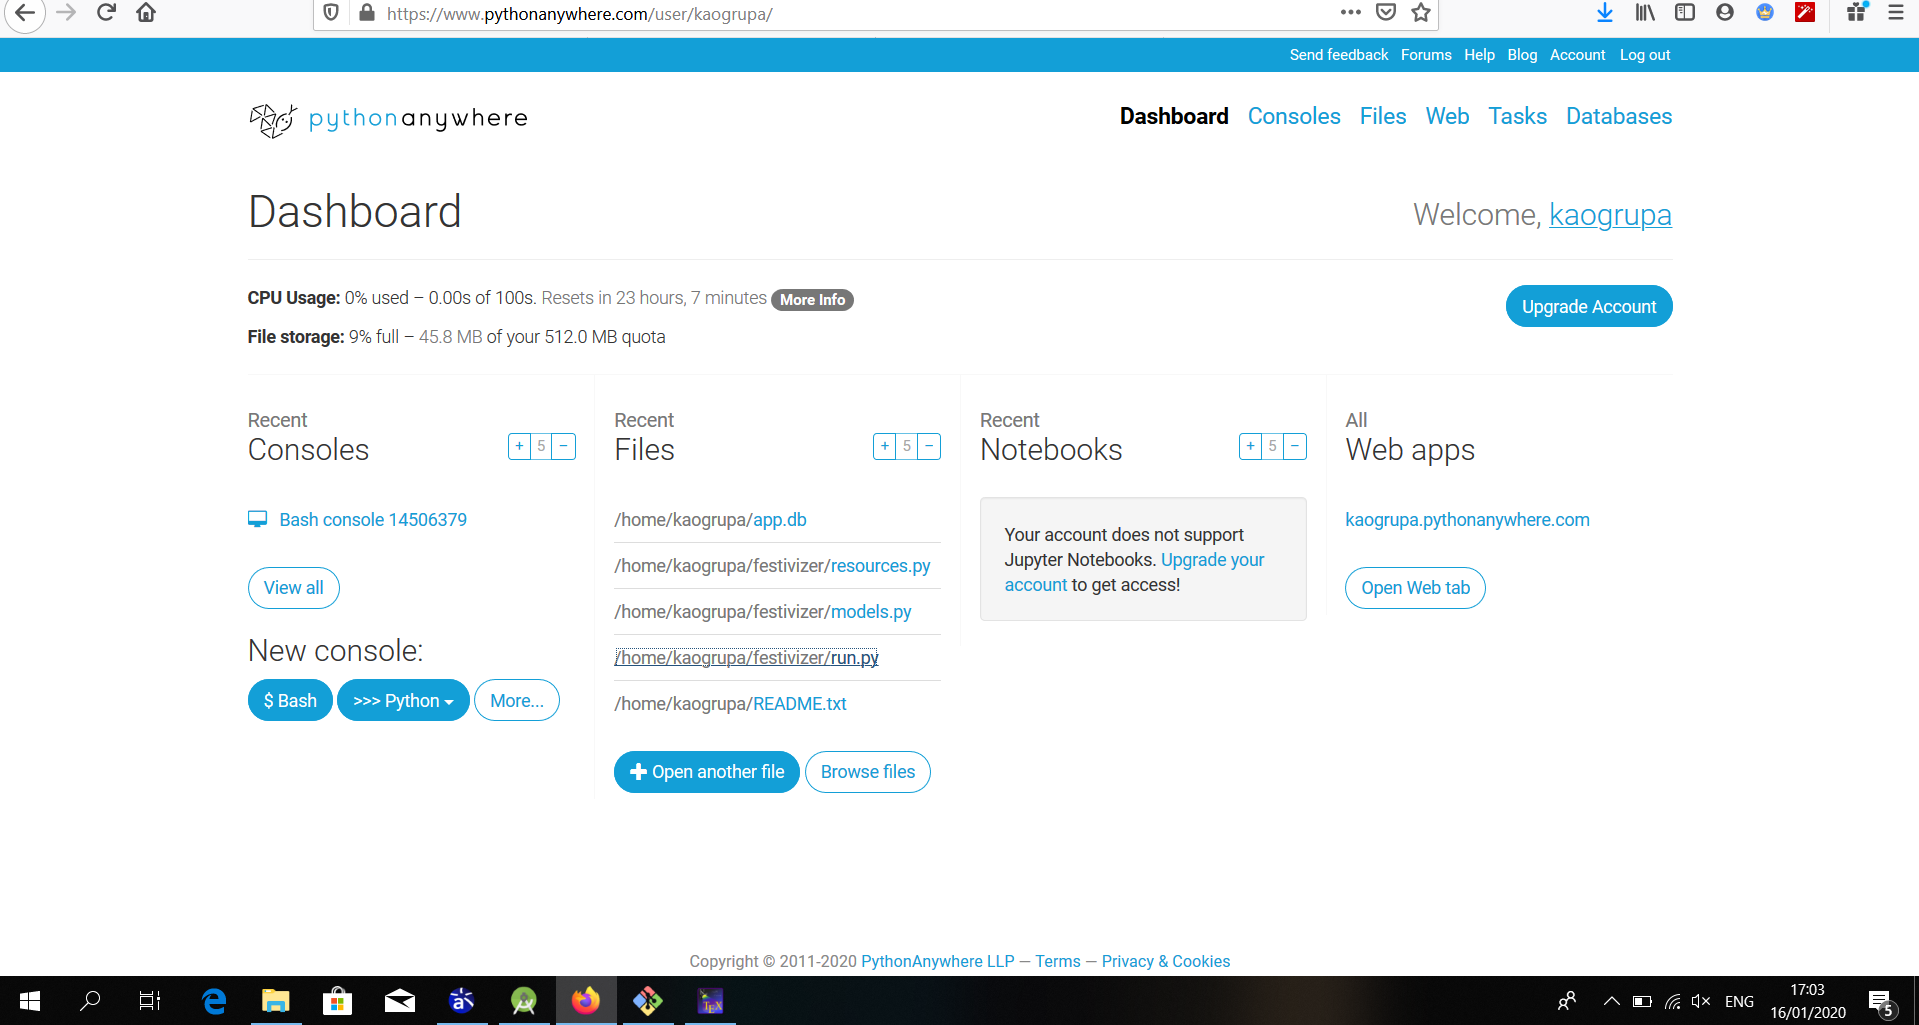
\includegraphics[width=\linewidth]{images/Deploy_2.png}
					\caption{Dashboard}
					\label{fig:deployment_2}
				\end{figure}
				
				Then click on the 'Open Web tab' button under the 'Web apps' title. Once there, click on the 'Add a new Web App' button.
				\begin{figure}[H]
					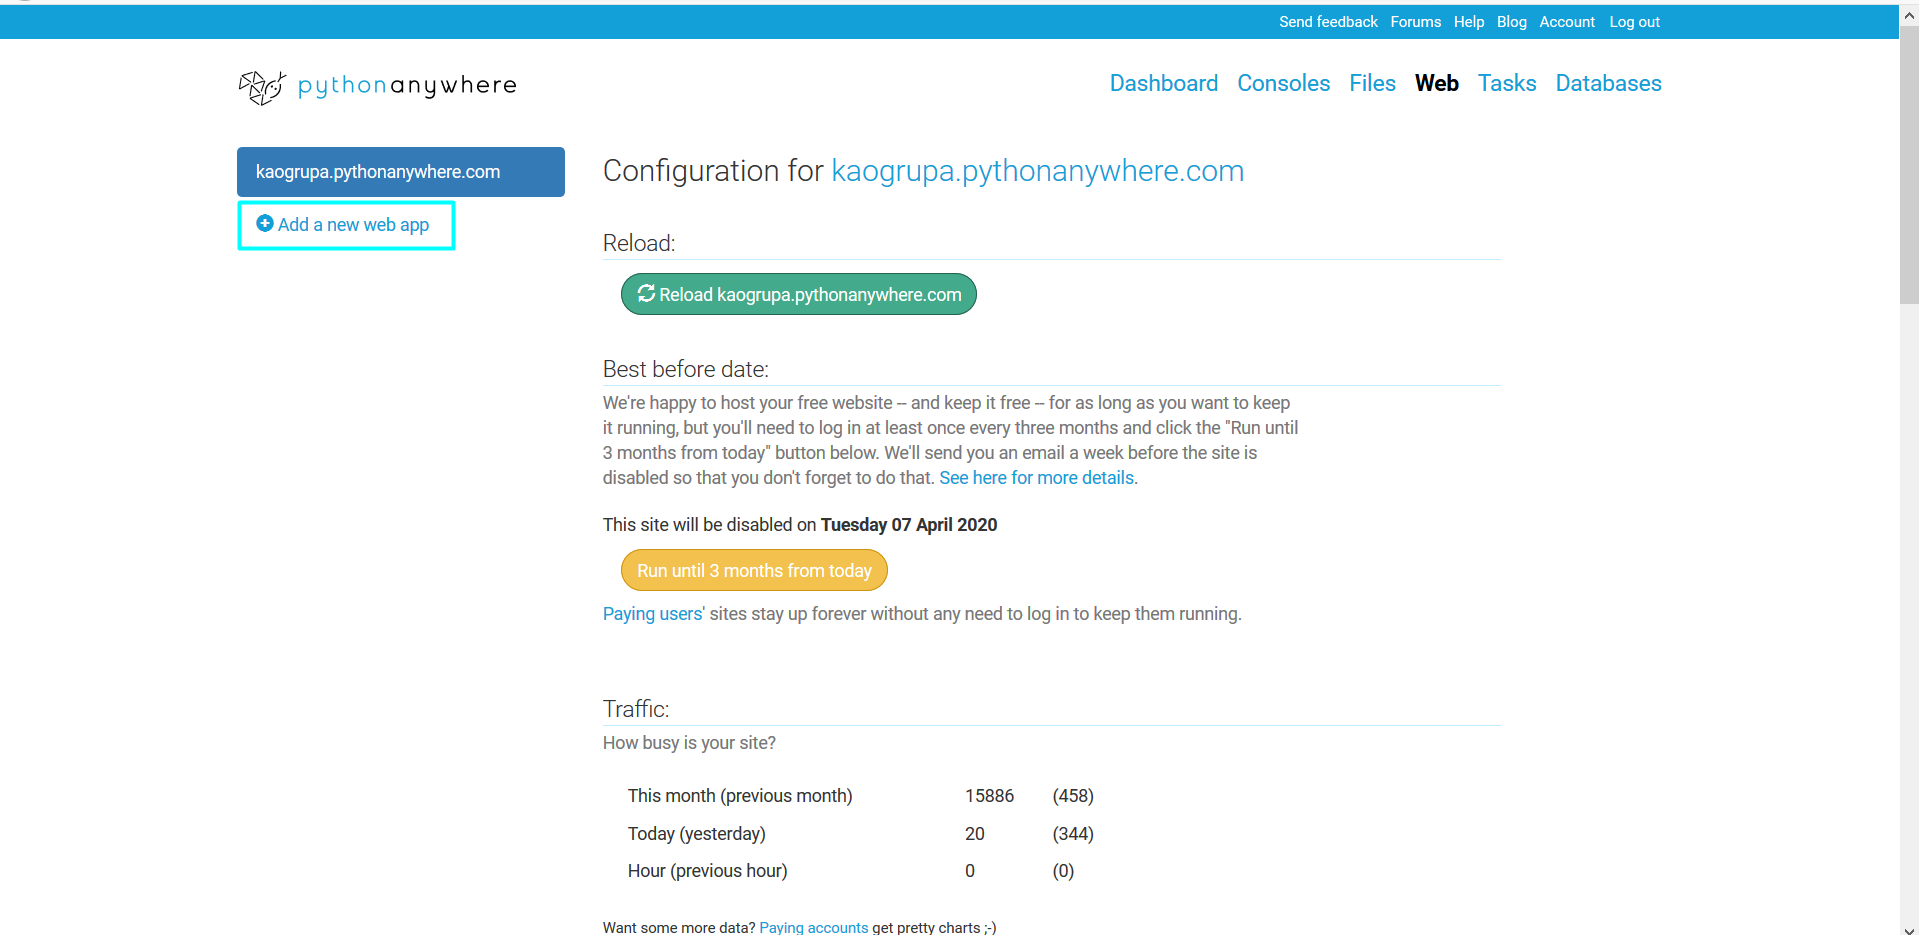
\includegraphics[width=\linewidth]{images/Deploy_3.png}
					\caption{Adding a new Web App}
					\label{fig:deployment_3}
				\end{figure}
				
				A wizard will appear on the right side, where you should select Flask. Python 3.6 is the minimum supported Python version. The default file flask_app.py will be generated. 
				
				Now the project is set up. All that is needed is to upload the files. Flask_app.py entry point file --> you should put into it the app.py code from git. Also upload the other files to the server. You should now be set up --> all that is left to do is to change the hardcoded kaogrupa URL in the application to point to your server. Once that is done, you have got your own back-end set up, and can comfortably change and experiment on the application.
				
				That is depictd on thee pictures below:
				\begin{figure}[H]
					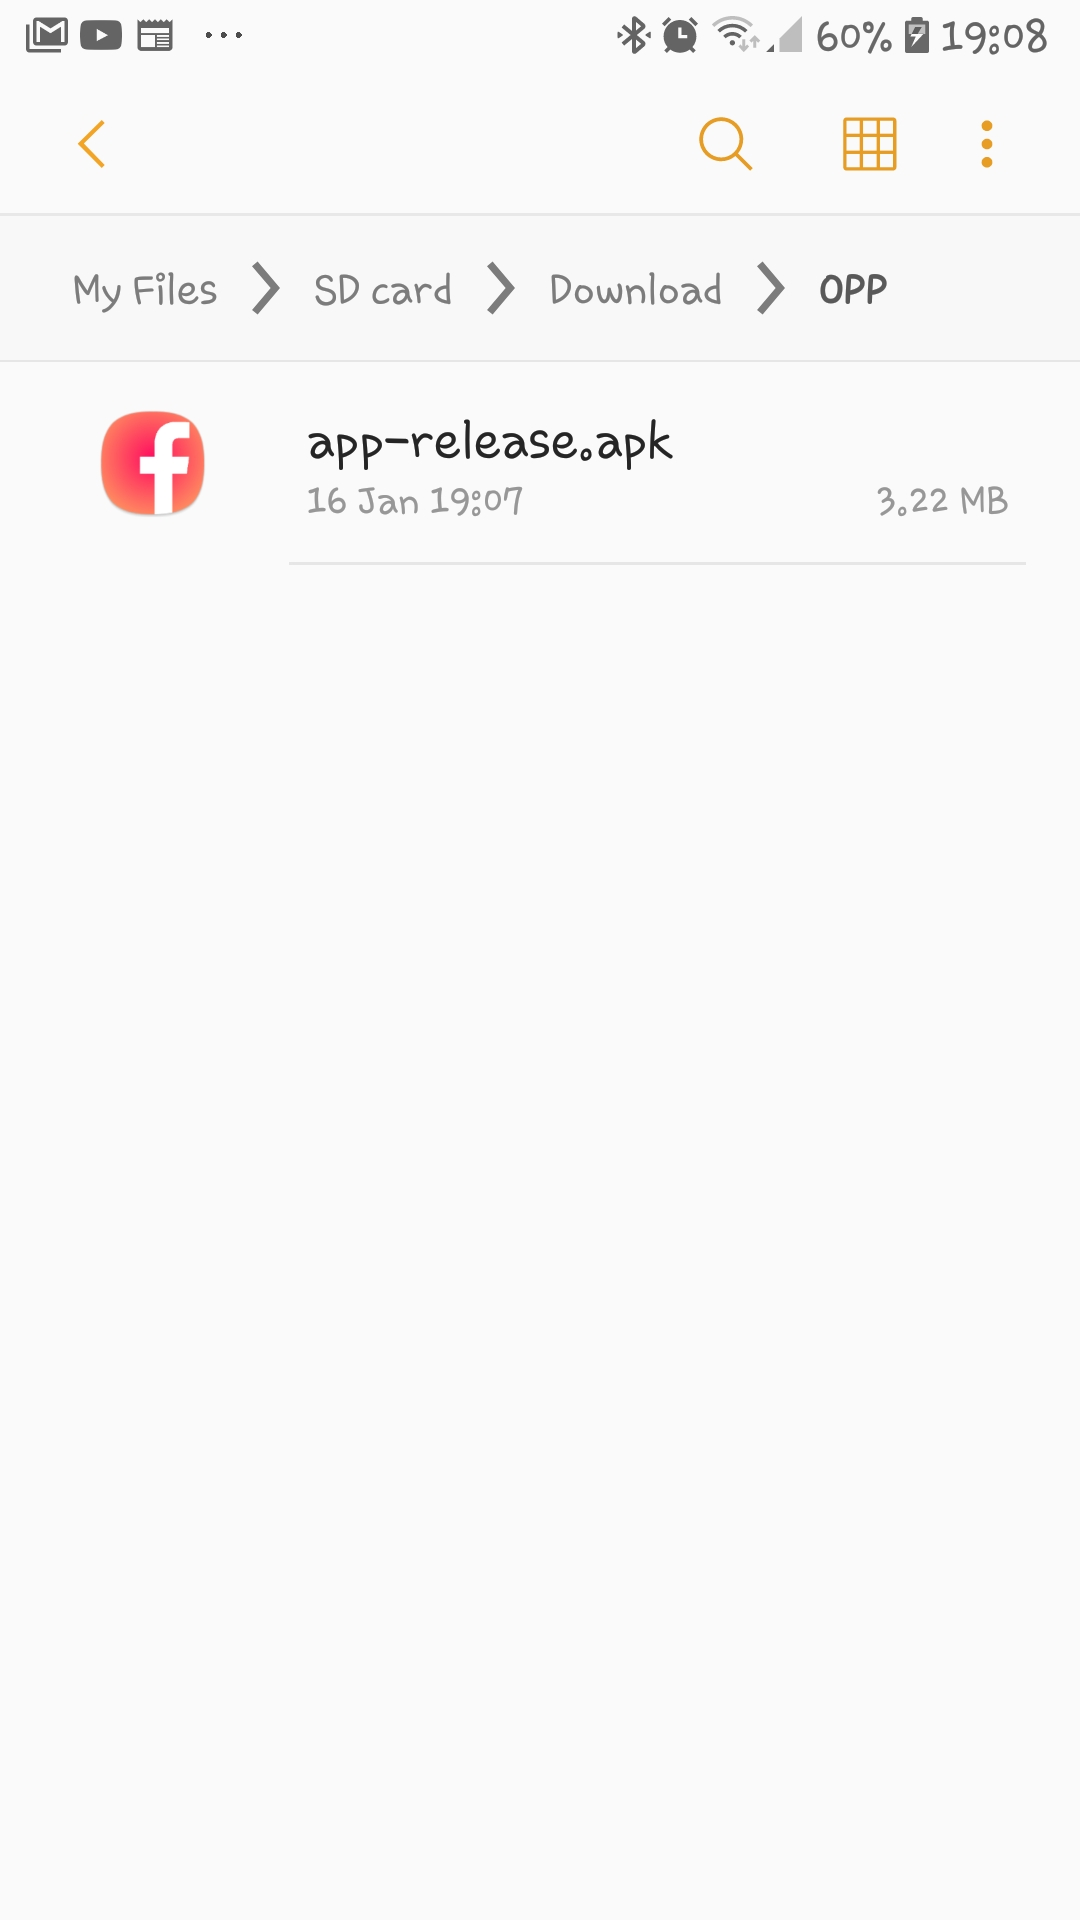
\includegraphics[width=\linewidth]{images/Android_1.png}
					\caption{Adding a new Web App}
					\label{fig:android_1}
				\end{figure}
			
				\begin{figure}[H]
					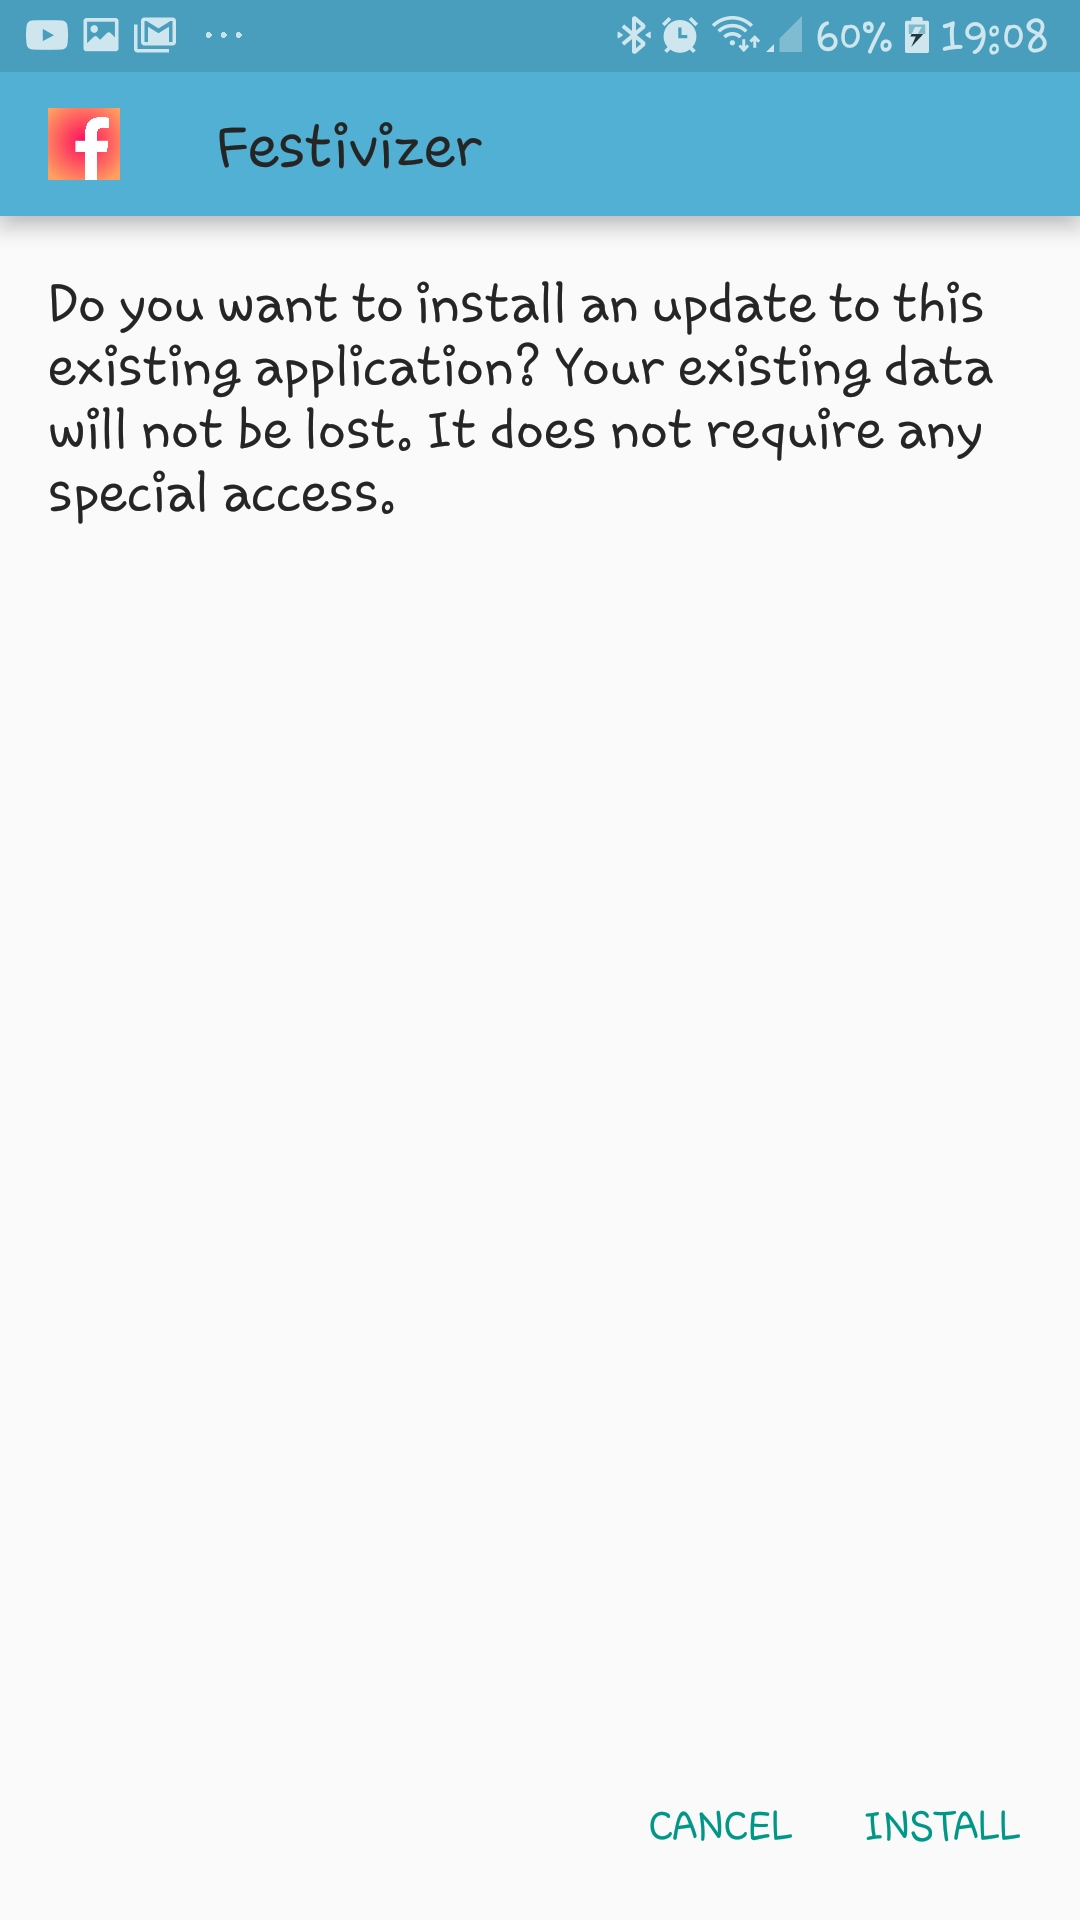
\includegraphics[width=\linewidth]{images/Android_2.png}
					\caption{Adding a new Web App}
					\label{fig:android_2}
				\end{figure}
			
				\begin{figure}[H]
					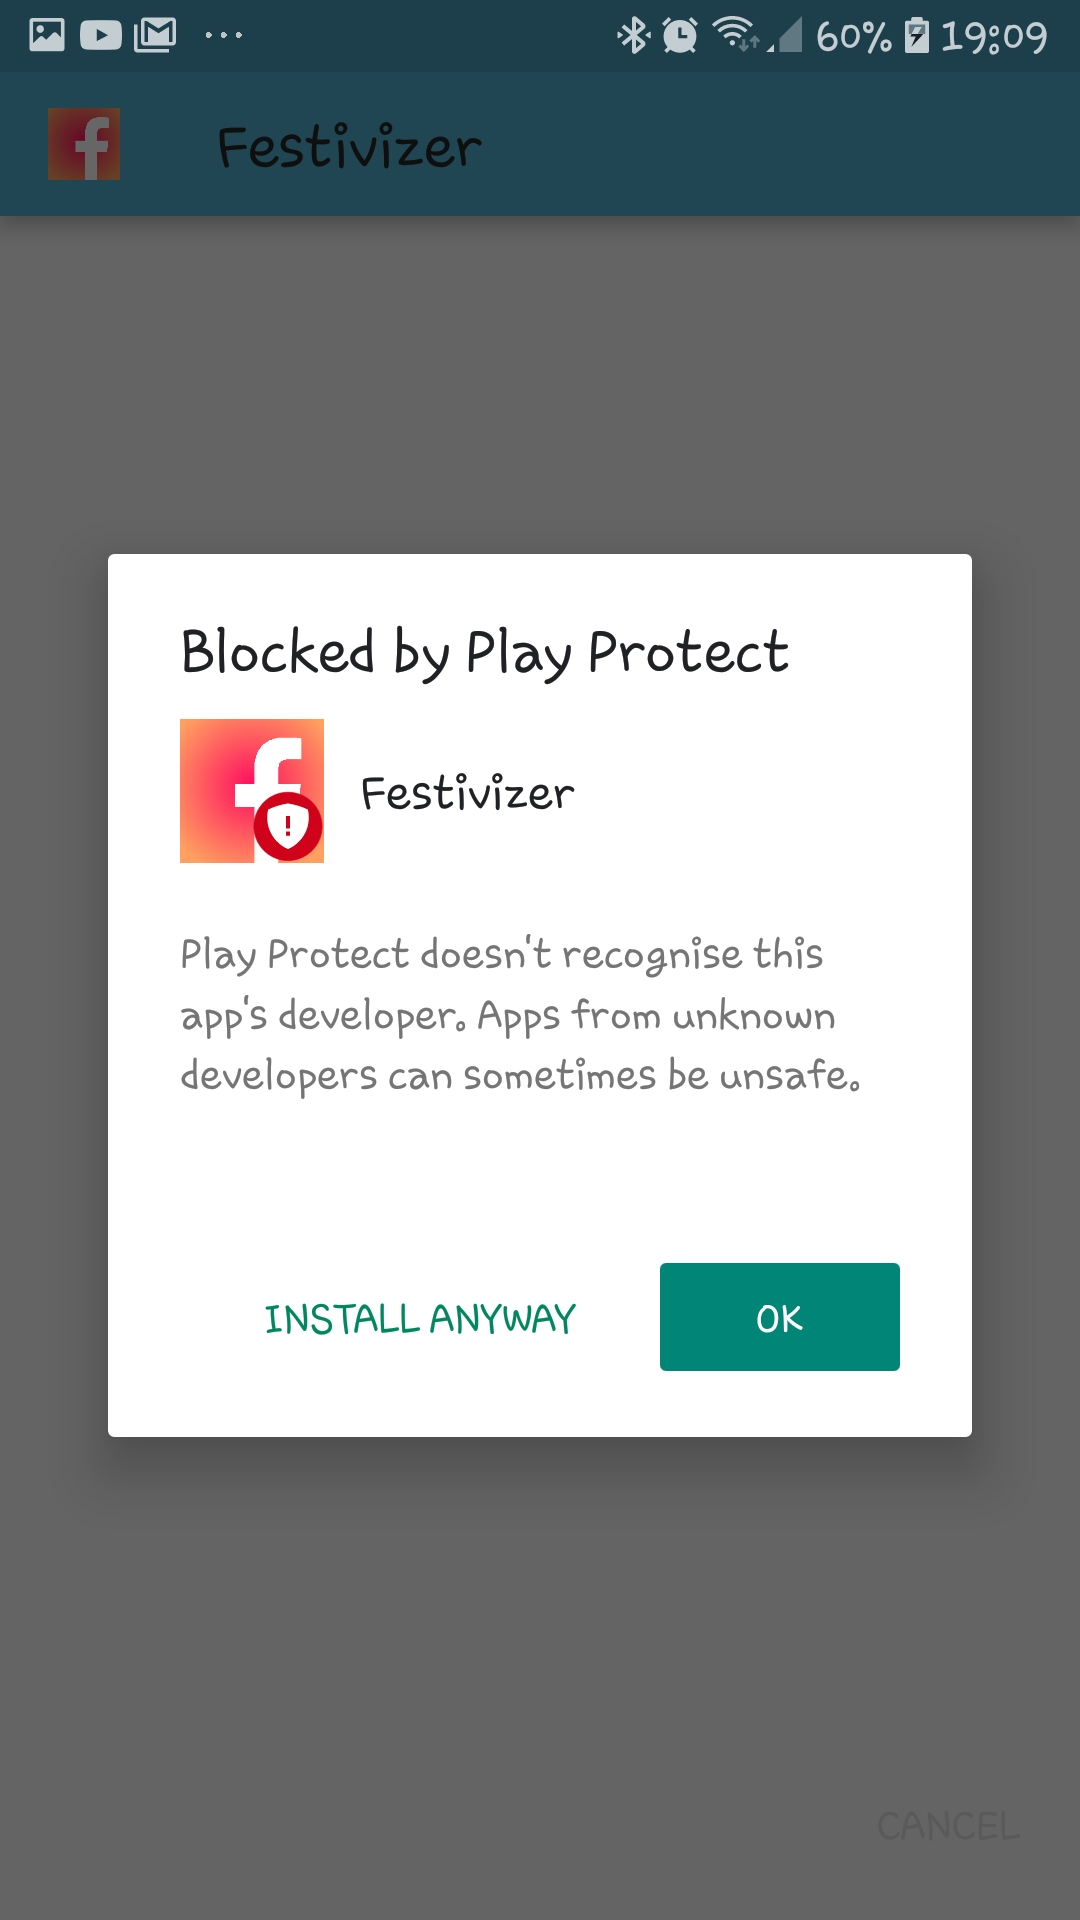
\includegraphics[width=\linewidth]{images/Android_3.png}
					\caption{Adding a new Web App}
					\label{fig:android_3}
				\end{figure}
			
			\eject 